\ifx \globalmark \undefined %% This is default.
\documentclass[a4paper,12pt]{report}

%%% PACKAGES %%%

\usepackage[french, english] {babel}	% langue principale
\usepackage[ansinew]{inputenc}
\usepackage[T1]{fontenc}		% Police contenant les caractères français
\usepackage{lmodern}			% plus beau
\usepackage[a4paper]{geometry} 
	\geometry{hscale=0.75,vscale=0.8,centering}

\usepackage[hidelinks]{hyperref} % pas de couleurs ici
%
\usepackage[natbibapa]{apacite}

%% Maths
\usepackage{amsfonts} % Equations etc
\usepackage{amsmath}
\usepackage{mathtools}
\usepackage{amssymb}

\usepackage{cleveref}

%% Itemizes
\usepackage{enumerate}
\usepackage{enumitem}

%% Dessins & Plots
\usepackage[pdftex]{graphicx} %Images dans le PDF
\usepackage{epstopdf}
\usepackage{color, xcolor}
\usepackage{chessboard}
\usepackage{booktabs,tabularx,multirow}
\usepackage[babel=true,kerning=true]{microtype}
%> Tikz
\usepackage{tikz}
\usepackage{hf-tikz}
\usetikzlibrary{ 
	calc,
	arrows,
	arrows.meta,
	automata, 
	shapes, 
	snakes, 
	positioning, 
	decorations,
	decorations.text,
	fit,
	matrix,
	mindmap
	}
	\tikzstyle{noeud-std}=[draw,fill=black,circle,inner sep=0pt,minimum size=7pt]% 7pt est la taille des cercles noirs
\usepackage{tkz-graph}
\newcommand{\tikzmark}[2]{\tikz[overlay,remember picture,baseline=(#1.base)] \node (#1) {#2};}
\newcommand{\Highlight}[1][submatrix]{%
    \tikz[overlay,remember picture]{
    \node[highlight,fit=(left.north west) (right.south east)] (#1) {};}
    }
\tikzset{%
  highlight/.style={rectangle,rounded corners,fill=ocre!50,draw,
    fill opacity=0.5,thick,inner sep=0pt}
}
\newcommand{\mytikzmark}[2]{\tikz[overlay,remember picture, baseline=(#1.base)] \node (#1) {#2};}


%% Meta
\usepackage{etoolbox}

% Debugging purposes: Catch when a reference is missing
\makeatletter
	\patchcmd{\@setref}{\bfseries ??}{{\color{red}[\texttt{\detokenize{ #3 }}]}}{}{%
	  \GenericWarning{}{Failed to patch \protect\@setref}}
	\patchcmd{\@citex}{\bfseries ?}{{\color{red}[\texttt{\detokenize{ #3 }}]}}{}{%{{\color{red}\texttt{\@citeb}}}{}{%
	  \GenericWarning{}{Failed to patch \protect\@citex}}
\makeatother

%% CUSTOM ENVIRONMENTS
% Packages
\usepackage{framed}
\usepackage{mdframed}
\usepackage[amsmath,thref, framed]{ntheorem}

%% Counters for theorem.
% The current choice is that all environments share a counter within chapters.
% It that regards, it becomes easy to navigate the document.

\newcounter{theo}[chapter]\setcounter{theo}{0}
\renewcommand{\thetheo}{\arabic{chapter}.\arabic{theo}}



% The following is adapted from https://texblog.org/2015/09/30/fancy-boxes-for-theorem-lemma-and-proof-with-mdframed/
% \newenvironment{name}[args]{begin_def}{end_def}
\newenvironment{generic_theo}[2][] % 2 arguments, and one is optional. The first argument will say if we have a Thm or somth, the second is the name of the thm.
	{% begin_def
		\refstepcounter{theo}%
		\ifstrempty{#2} % looking at the name of the thm
		{	
			\mdfsetup{
				frametitle={
					\tikz[baseline=(current bounding box.east),outer sep=0pt]
					\node[anchor=east,rectangle,fill=white!20, draw = black!20, line width = 2pt]
					{\strut #1~\thetheo};}
			} % The #1 will say Theorem, or other.
		}
		{
			\mdfsetup{
				frametitle={
				\tikz[baseline=(current bounding box.east),outer sep=0pt]
				\node[anchor=east,rectangle,fill=white!20, draw = black!20, line width = 2pt]
				{\strut #1~\thetheo:~#2};}
			}
		}
		\mdfsetup{innertopmargin=10pt,linecolor=black!20,
					linewidth=2pt,topline=true,
					frametitleaboveskip=\dimexpr-\ht\strutbox\relax
				}
\begin{mdframed}[]\relax}{\end{mdframed}}


%% Proofs (slightly different)
\newenvironment{generic_proof}[2][] % 2 arguments, and one is optional. The first argument will say if we have a Thm or somth, the second is the name of the thm.
	{% begin_def
		\refstepcounter{theo}%
		\ifstrempty{#2} % looking at the name of the thm
		{	
			\mdfsetup{
				frametitle={
					\tikz[baseline=(current bounding box.east),outer sep=0pt]
					\node[anchor=east,rectangle,fill=black!20]
					{\strut #1~\thetheo};}} % The #1 will say Theorem, or other.
		}
		{
			\mdfsetup{
				frametitle={
				\tikz[baseline=(current bounding box.east),outer sep=0pt]
				\node[anchor=east,rectangle,fill=black!20]
				{\strut #1~\thetheo:~#2};}}
		}
		\mdfsetup{innertopmargin=10pt,linecolor=black!20,
					linewidth=1pt,topline=true,
					frametitleaboveskip=\dimexpr-\ht\strutbox\relax
				}
\begin{mdframed}[]
}{\end{mdframed}}

%% Examples/Exercices
\newenvironment{generic_ex}[2][] % 2 arguments, and one is optional. The first argument will say if we have a Thm or somth, the second is the name of the thm.
	{% begin_def
		\refstepcounter{theo}%
		\ifstrempty{#2} % looking at the name of the thm
		{	
			\mdfsetup{
				frametitle={
					\tikz[baseline=(current bounding box.east),outer sep=0pt]
					\node[anchor=east,rectangle,fill=black!20]
					{\strut #1~\thetheo};}} % The #1 will say Theorem, or other.
		}
		{
			\mdfsetup{
				frametitle={
				\tikz[baseline=(current bounding box.east),outer sep=0pt]
				\node[anchor=east,rectangle,fill=black!20]
				{\strut #1~\thetheo:~#2};}}
		}
		\mdfsetup{innertopmargin=10pt,linecolor=black!20,
					linewidth=1pt,topline=true,
					frametitleaboveskip=\dimexpr-\ht\strutbox\relax
				}
\begin{mdframed}[]
}{\end{mdframed}}



% The different environments that we need (Main stuff are highlighted.
\newenvironment{theorem}[1][]{\begin{generic_theo}[Theorem]{#1}}{\end{generic_theo}}
\newenvironment{lemma}[1][]{\begin{generic_theo}[Lemma]{#1}}{\end{generic_theo}}
\newenvironment{definition}[1][]{\begin{generic_theo}[Definition]{#1}}{\end{generic_theo}}
\newenvironment{notation}[1][]{\begin{generic_theo}[Notation]{#1}}{\end{generic_theo}}
\newenvironment{proposition}[1][]{\begin{generic_theo}[Proposition]{#1}}{\end{generic_theo}}
\newenvironment{procedure}[1][]{\begin{generic_theo}[Procedure]{#1}}{\end{generic_theo}}
\newenvironment{hypothese}[1][]{\begin{generic_theo}[Hypothesis]{#1}}{\end{generic_theo}}


% These ones, let's not overblow them
% The true reason why I'm doing this is that there may be floats in Exercices and Examples...
% You can't have  begin{figures} in mdframed env, it crashes.
%\newtheorem{notation}[theo]{Notation}
\newcounter{axiomc}[chapter]\setcounter{axiomc}{0}
\renewcommand{\theaxiomc}{\arabic{chapter}.\arabic{axiomc}}

\newtheorem{axiom}[axiomc]{Axiom}
\newtheorem{proof}[theo]{Proof}
\newtheorem{exercise}[theo]{Exercise}
\newtheorem{example}[theo]{Example}



%% CUSTOM Commands

% Identify TAs
\newcommand{\TAone}{Matthew}
\newcommand{\TAtwo}{Beno\^it}

\newcommand{\reels}{\mathbb{R}}

\DeclareMathOperator*{\argmin}{arg\,min}
\DeclareMathOperator*{\argmax}{arg\,max}

% Nice brackets
\newcommand\parent[1]{\left(#1\right)}
\newcommand\abs[1]{\left\lvert#1\right\rvert}
\newcommand\norm[1]{\left\lVert#1\right\rVert}
\newcommand\bracket[1]{\left\{#1\right\}}
\newcommand\squared[1]{\left[#1\right]}

\DeclarePairedDelimiter{\floor}{\lfloor}{\rfloor}
\DeclarePairedDelimiter{\ceil}{\lceil}{\rceil}
\usepackage{eurosym}
\usepackage{siunitx}
\DeclareSIUnit{\EUR}{\text{\euro}}
\sisetup{
  per-mode = fraction,
  inter-unit-product = \ensuremath{{}\cdot{}},
}



\usepackage{textcomp}
\let\texteuro\euro





	\begin{document} %% Crashes if put after (one of the many mysteries of LaTeX?).
\else
\fi



\chapter{Refinements of Equilibria}
\label{chap:Refinements}
{\large{\itshape
``Have no fear for perfection, you will never reach it.''} --- Salvador Dali.\\}
  {\small{\itshape
Chapter based on pages 213 to 232 of the book  ``Game theory - Analysis of conflict'' by R. Myerson.}\\
}

So far, our goal has been to understand the behaviour of rational and intelligent agents in a finite game, where the players take actions, without negotiation, with the goal of maximizing their payoffs. Decision  theory (Chapter \ref{chap:Decision}) and the Utility Maximization Theorem brought  valuable insights to that end, that lead to the development of the Nash Equilibrium (Chapter \ref{chap:Nash}). This chapter is the last one to be situated in this context.\\
At the end, Nash Equilibria have drawbacks in that they don't alone, capture the rational behaviour of players. But they are computed from the strategic form, a compact representation of a game. Sequential Equilibria (Chapter \ref{chap:Seq}) capture the  sequential rationality of players (a rational player wants to maximize its payoff at every move, not all Nash equilibria allow for this) are computed from the extensive form of a game. \\
In this chapter, we investigate other definitions of equilibria. Namely, we will describe the Sub-game perfect equilibrium, the Perfect Equilibrium. Ending this chapter, we situate these definitions relative to one another, providing a unifying picture.
\section{The Sub-game perfect equilibrium}

When playing rock-paper-scissors, the one and only Nash equilibrium of the game is to play each move with probability $1/3$. If we played the game 10 times in a row, what should we do on the 10th game?
The answer is easy: regardless of the outcomes of the previous 9 games, the 10th game being nothing else than a rock-paper-scissors game, we should again play each move with probability $1/3$.\\
In this section, we tackle situations where a player, at some point in the game, has to make decisions knowing that the payoffs he will get from these decisions is actually independent of the past decisions made in the game (which comprise both his and his opponent's actions).
To do so, we define the concept of a \emph{subgame} of a game in strategic form. Note that we here make use of the formalism of Chapter \ref{chap:Seq} describing extensive form trees (Definition \ref{chap4:def:GameInExtForm}). An example is shown afterwards.
\begin{definition}[Subroots and subgames]
Consider a game in extensive form $\Gamma^e$.
For any node $x \in X$, let $F(x) \subseteq X$ be the set of nodes in the subtree rooted at $x$. \\
A \emph{subroot} of the game is a node $x \in X$ such that, for any information state $s \in S$, we have
$$\text{either } Y_s \cap F(x) = \emptyset, \text{ or } Y_s \cap F(x) = Y_s.$$
Given a subroot $x \in X$ of $\Gamma^e$, a \emph{subgame} rooted at $x$ is the game obtained by removing from $\Gamma^e$ all nodes not in $F(x)$.
\end{definition}

\begin{example}
Consider the following game, from Example \ref{ch4:ex:badEqu}:
\begin{figure}[!ht]
\begin{center}
\begin{tikzpicture}
\node[noeud-std] (noeud0) {}
	[sibling distance=4cm]
	child[level distance=1cm]{node[noeud-std,fill=white] (noeud1){}}
	child[level distance=1cm] {node[noeud-std] (noeud2) {}
		[sibling distance=3cm]
			child[level distance=1cm]{node[noeud-std,fill=white] (noeud3){}}
			child[level distance=1cm]{node[noeud-std,fill=white] (noeud4){}}
		}

    ;

\node[above=5pt] at (noeud0) {$1.a$};
\node[above=-25pt] at (noeud0) {$X_0$};
\node[above left] at ($(noeud0)!{0.4}!(noeud1)$) {\texttt{$y_1$}};
\node[above right] at ($(noeud0)!{0.4}!(noeud2)$) {\texttt{$x_1$}};
\node[above=-20pt] at (noeud1) {$1\, / \, 9$};
\node[above=5pt] at (noeud2) {$2.b$};
\node[above=-25pt] at (noeud2) {$X_1$};
\node[above left] at ($(noeud2)!{0.4}!(noeud3)$) {\texttt{$y_2$}};
\node[above right] at ($(noeud2)!{0.4}!(noeud4)$) {\texttt{$x_2$}};
\node[above=-20pt] at (noeud3) {$0\, / \, 2$};
  \node[above=-20pt] at (noeud4) {$2\, / \, 3$};
\end{tikzpicture}
\end{center}
\end{figure}

Both the nodes $X_0$ and $X_1$ are subroot of the game.
The big idea is that at both of these nodes, the payoffs depend only on future actions.
\label{ch5:ex:subgame1}
\end{example}
This allows us to define the concept of subgame perfect equilibrium.
\begin{definition}
A \emph{subgame perfect equilibrium} of an extensive form game $\Gamma^e$ is any Nash equilibrium of $\Gamma^e$ such that the restriction of this equilibrium to any subgame is a Nash equilibrium of that subgame.
\end{definition}
\begin{theorem}
The set of subgame perfect equilibria is non-empty.
\end{theorem}
At a subgame perfect equilibrium, a player will play rationally at every subgame.
If a subgame perfect equilibrium is a Nash equilibrium, all Nash equilibria are not subgame perfect.
\begin{example}
The strategic form of the game of Example \ref{ch5:ex:subgame1}
is
\begin{center}
\begin{tabular}{c|cc}
& $x_2$ & $y_2$ \\
\hline
$x_1$ & 2,  3 & 0, 2 \\
$y_1$ & 1, 9 & 1, 9
\end{tabular}
\end{center}
There are two Nash equilibria to that game, which are $([x_1], [x_2])$ and $([y_1], [y_2])$. However, only the first one is subgame perfect. Indeed, if we consider the subgame rooted at node $X_1$, whose strategic form is
\begin{center}
\begin{tabular}{c|cc}
$X_1$ subgame & $x_2$ & $y_2$ \\
\hline
$\cdot$ & 2, 3 & 0, 2 \\
\end{tabular}
\end{center}
we see that the payoffs depend only on the move of player 2. Here, $x_2$ dominates $y_2$. Thus, the restriction of the equilibrium $([x_1], [x_2])$ to the subgame rooted at $X_1$ is an equilibrium at that subgame.\\
\end{example}
One of the main flaw in the definition of subgame-perfect equilibria is that they are highly sensitive to the modelling of the game, as shown next.
\begin{example}
Consider this variant of the game of Example \ref{ch5:ex:subgame1}.

\begin{figure}[!ht]
\begin{center}
\begin{tikzpicture}
\node[noeud-std] (noeud0) {}
	[sibling distance=4cm]
	child[level distance=1cm]{node[noeud-std] (noeud1){}
		child[level distance=1cm] {node[noeud-std,fill=white] (noeud7) {} }
	}
	child[level distance=1cm] {node[noeud-std] (noeud2) {}
		[sibling distance=3cm]
			child[level distance=1cm]{node[noeud-std] (noeud3){}
				child[level distance=1cm] {node[noeud-std,fill=white] (noeud5) {} }
			}
			child[level distance=1cm]{node[noeud-std] (noeud4){}
				child[level distance=1cm] {node[noeud-std,fill=white] (noeud6) {} }
			}
		}

    ;

\node[above=5pt] at (noeud0) {$1.a$};
\node[above=-25pt] at (noeud0) {$X_0$};
\node[above left] at ($(noeud0)!{0.4}!(noeud1)$) {\texttt{$y_1$}};
\node[above right] at ($(noeud0)!{0.4}!(noeud2)$) {\texttt{$x_1$}};
\node[above=-20pt] at (noeud7) {$1\, / \, 9$};
\node[above=5pt] at (noeud2) {$2.b$};
\node[above=-25pt] at (noeud2) {$X_1$};
\node[above left] at ($(noeud2)!{0.4}!(noeud3)$) {\texttt{$y_2$}};
\node[above right] at ($(noeud2)!{0.4}!(noeud4)$) {\texttt{$x_2$}};
\node[above=-20pt] at (noeud5) {$0\, / \, 2$};
  \node[above=-20pt] at (noeud6) {$2\, / \, 3$};
  \node[ left] at ($(noeud1)!{0.4}!(noeud7)$) {\texttt{$d$}};
  \node[ left] at ($(noeud3)!{0.4}!(noeud5)$) {\texttt{$d$}};
  \node[ left] at ($(noeud4)!{0.4}!(noeud6)$) {\texttt{$d$}};
  \node[above=5pt] at (noeud1) {$1.c$};
    \node[above=5pt] at (noeud3) {$1.c$};
       \node[above=5pt] at (noeud4) {$1.c$};
\end{tikzpicture}
\end{center}
\end{figure}


The game now has only 1 subroot (which is $X_0$), thus both the equilibria $([x_1,d], [x_2])$ and $([y_1,d], [y_2])$ are subgame perfect.


This shows that simply by adding one more step to the game (with no effects at all on the outcomes), subgame-perfect equilibria may no longer help us detect irrational Nash Equilibria.
\end{example}

Even if they are sensitive to the modelization, subgame-perfect equilibria remain  particularly relevant when addressing \emph{Repeated Games} (see Chapter \ref{chap:Rep}).

\section{The Perfect equilibrium}

Perfect equilibria, as we will explain, are very robust by definition. They are also known as \emph{Trembling Hand perfect equilibria}.\\
\begin{definition}
A perfect equilibrium for a game in strategic form $\Gamma(N,C,u)$ is a strategy profile $\sigma \in \times_{i \in N} \Delta (C_i)$ such that there is a sequence of strategy profiles $ (\sigma^k)_{k = 1}^\infty$ satisfying
\begin{itemize}
\item $\sigma^k \in \times_{i \in N} \Delta^0 (C_i)$ (non-zero probability of playing any strategy),
\item $\lim_{k \rightarrow \infty} \sigma^k = \sigma$ (sequence converges to equilibrium),
\item $ \sigma_i \in \argmax_{\tau_i \in \Delta(C_i)}u_i(\sigma^k_{-i}, \tau_i), \forall i \in N, k = 1,2, \cdots $ (equilibrium is best response to all strategies in the sequence).
\end{itemize}
\label{ch5:def:perfectEq}
\end{definition}
The concept shows some resemblance with the one of sequential equilibrium (Definitions \ref{ch4:def:StrongCons} and \ref{ch4:def:SeqEq}). A sequential equilibrium requires a fully consistent belief vector. The two concepts embed within their definition the idea that the equilibrium strategy is obtained as the limit of strategies which put non-zero probabilities on every move. The difference here lies in the fact that the perfect equilibrium strategy must \emph{additionally} be a best response to all the strategies in the sequence.
%As an immediate effect, we may prove (left as an exercise) that a perfect equilibrium may never be composed of \emph{weakly dominated strategies}.
\begin{example}
Consider the following game:
\begin{center}
\begin{tabular}{c | c  c}
& $x_2$ & $y_2$ \\
\hline
$x_1$ & 2, 2 & -1, 2 \\
$y_1$ & 2, -1 & 0, 0
\end{tabular}
\end{center}
For both players, the strategy $x$ is weakly dominated by the strategy $y$.
Nevertheless, amongst the two Nash equilibria of the game $([x_1],[x_2])$ and $([y_1],[y_2])$, the first uses weakly dominated strategies. \\
Let us now verify if these equilibria are \emph{perfect}.
Take  any randomized strategy of player 2, say $\sigma_2 = (\alpha [x_2] + 1- \alpha [y_2])$. If $\alpha \in ]0,1[$, $\sigma_2 \in \Delta^0(C_2)$. For player 1, the best response to $\sigma_2$ is always $y_1$, which grants him a payoff of $2 \alpha$ (compared to $3\alpha - 1 < 2 \alpha$ for $\alpha \leq 1$).\\
Since the game is symmetric and that  best response of player 1 to any strategy in $\Delta^0(C_2)$ is $y_1$, we conclude that $([y_1], [y_2])$ is a perfect equilibrium, but not $([x_1],[x_2])$.
\end{example}

The previous example illustrates one of the drawbacks of perfect equilibria, in that players may no longer consider equilibria in weakly dominated strategies. Nevertheless, in many games, doing so makes a lot of sense!\\
Perfect equilibria, however, do come with a good news.
\begin{theorem}
For any \emph{extensive form} game $\Gamma^e$, if the behavioural strategy profile $\sigma$  is a perfect equilibrium for the multi-agent representation of $\Gamma^e$, then there exists a strongly consistent belief vector $\pi$ such that $(\sigma, \pi)$ is a sequential equilibrium.
\end{theorem}

Moreover, the existence of a perfect equilibria is guaranteed
\begin{theorem}
Given a game in strategic form, the set of all perfect equilibria is non-empty.
\end{theorem}
\begin{example}
We go back to the signalling game of Example \ref{ch4:ex:signalling}.
We saw that the game had 3 Nash equilibria, which all match sequential equilibria, but two of them were composed of weakly dominated strategies. \\
Consequently, amongst the 3, only one can correspond to a perfect equilibrium.
Interestingly, it is the one that corresponds to always choosing the relax option for player 1, and always choosing the hire option for player 2...
\end{example}

\subsection{Refinement - proper equilibrium}

In the above, we learnt that a perfect equilibria of a multi-agent representation corresponds to a sequential equilibria. The result is actually quite surprising: we can find a \emph{sequentially rational} set of moves without even looking at the extensive form of a game! We still need to consider the multi-agent form though.

The concept of perfect equilibrium can be further refined.
\begin{definition}
A \emph{proper} equilibrium for a game in strategic form $\Gamma(N,C,u)$ is a strategy profile $\sigma \in \times_{i \in N} \Delta (C_i)$ such that there is a sequence of strategy profiles $ (\sigma^k)_{k = 1}^\infty$, and a sequence $(\epsilon_k)_{k = 1}^{\infty}$ satisfying
\begin{itemize}
\item $\sigma^k \in \times_{i \in N} \Delta^0 (C_i)$ (non-zero probability of playing any strategy),
\item $\lim_{k \rightarrow \infty} \sigma^k = \sigma$ (sequence converges to equilibrium),
\item $ \sigma_i \in \argmax_{\tau_i \in \Delta(C_i)}u_i(\sigma^k_{-i}, \tau_i), \forall i \in N, k = 1,2, \cdots $ (equilibrium is best response to any strategy in the sequence),
\end{itemize}
and in addition,
\begin{itemize}
\item $\forall k, \forall i \in N, \forall c_i, e_i \in C_i: \, u_i(\sigma_{-i}^k, [c_i]) < u_i(\sigma_{-i}^k, [e_i]) \Rightarrow \sigma^k_i(c_i) < \epsilon_k \sigma_i(e_i)$ (penalize bad moves),
\item $\lim_{k \rightarrow \infty} e_k = 0$ (penalty vanishes at equilibrium).
\end{itemize}
\label{ch5:def:properEq}
\end{definition}

The fun thing with proper equilibria is that we can now detect sequential equilibria of a game \emph{from its strategic form!}

\begin{theorem}
Consider a game $\Gamma^e$ in extensive form with a normal representation $\Gamma(N,C,u)$.
If $\sigma$ is a proper equilibrium of $\Gamma$, then there is a behavioural representation $\tau$ of $\sigma$ and a belief vector $\pi$ such that $(\tau, \pi)$ is a sequential equilibrium of $\Gamma^e$.
\end{theorem}

This has actually deep repercussions. One of the problems with the strategic form is that it may represent several games in extensive form.
Consequently: an equilibrium for a game $\Gamma$ can be perfect if and only if there is an extensive form game, whose strategic form is $\Gamma$, where a behavioural representation of the equilibrium is sequential.


\section{Equilibria in non-cooperative games: unifying picture}

Given a game in extensive form (its more general representation), we are interested in figuring out the moves that could be played by rational and intelligent player. Based on the axioms of decision theory, and the normal form representation, the concept of Nash equilibrium was presented first.\\
Any game always has at least one \emph{Nash Equilibrium}, and rational players need to play at Nash equilibria. However, the reverse is not true: not all Nash Equilibrium correspond to strategies rational players may play.
The problem with Nash Equilibria is that players make several sequential decisions  in a game, and seek to maximize their payoffs at every stage. In this context, \emph{Subgame perfect} equilibria appear naturally. They correspond to Nash Equilibria whose restriction to any subgame is also a Nash Equilibria. Any game always has at least one Subgame perfect equilibrium!
One step further is the Sequential Equilibrium. Here, players not only make rational moves at the beginning of the game (Nash) or at the beginning of each subgame (Subgame perfect), but at \emph{every information state}. Again, any game always has at least one Sequential Equilibria. These equilibria are described in terms of behavioural strategies, and their computation relies on the extensive form of a game. Sequential equilibria are perhaps the solution concepts that capture the notion of rationality the best. At a sequential equilibria, player motivate their actions through their beliefs vectors: from their point of view, their actions are rational at every information state.
Finally, we discussed perfect equilibria and proper equilibria.
They offer cautious definitions for equilibria, where a player should play a strategy which is a best response to a sequence of randomized strategies, that put positive probabilities on all actions. They have some interesting theoretical properties: both are guaranteed to exists, a perfect equilibrium of the multi-agent representation corresponds to a sequential equilibrium, and so does a proper equilibrium of strategic form.

The relation between the above mentioned types of  equilibria is shown on Figure \ref{ch5:fig:equilibriaRelation}.

\begin{figure}[!ht]
\centering
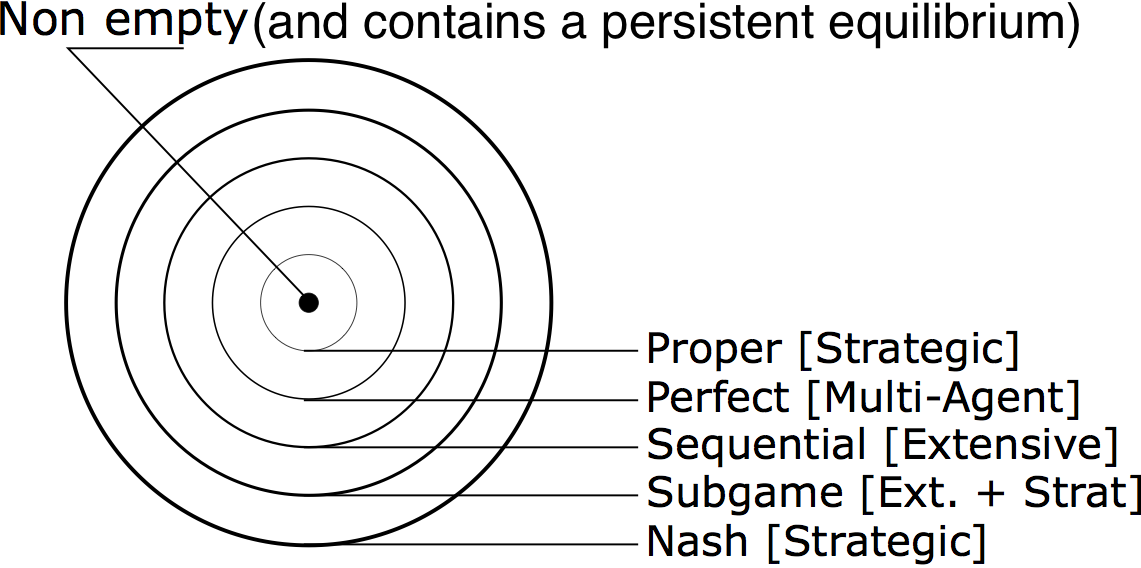
\includegraphics[scale=0.7]{equilibriaRelationMOD.png}
\caption{Inclusion relations between different types of equilibria.}
\label{ch5:fig:equilibriaRelation}
\end{figure}





%%

\ifx \globalmark \undefined %% This is default.
\bibliographystyle{plain}
\bibliography{../gametheorybibliography}
	\end{document}
\else

\fi
